% Corpus document: a Beamer deck (DESIGN.md §8). Beamer's class and theme loading is its own
% kind of heavy, and overlays multiply pages, so it times differently from any article.
\documentclass[aspectratio=169]{beamer}
\usetheme{Madrid}
\usecolortheme{beaver}
\usepackage{tikz}
\usetikzlibrary{arrows.meta,positioning}
\usepackage{booktabs}

\title{Warm Builds Are Cheap}
\subtitle{Measuring local \LaTeX{} latency}
\author{A.~Author}
\institute{Department of Writing Tools}
\date{September 2026}

\begin{document}

\begin{frame}
  \titlepage
\end{frame}

\begin{frame}{Outline}
  \tableofcontents
\end{frame}

\section{Problem}

\begin{frame}{Where the time goes}
  \begin{itemize}
    \item<1-> Queue wait on a shared server
    \item<2-> Container start
    \item<3-> The compile itself
    \item<4-> Transfer and render
  \end{itemize}
  \only<4>{\alert{Only the third survives going local.}}
\end{frame}

\begin{frame}{The loop}
  \centering
  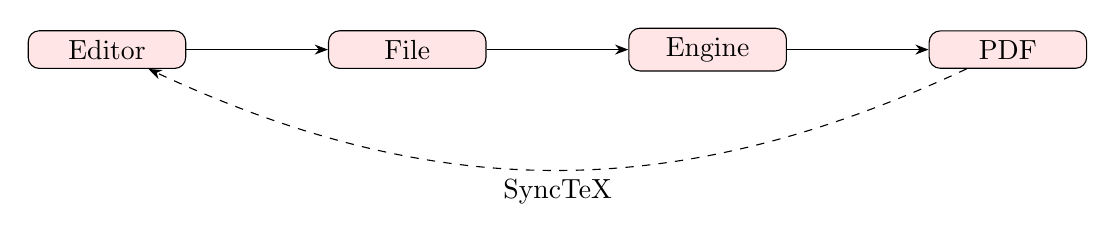
\begin{tikzpicture}[node distance=1.8cm, box/.style={draw, rounded corners, fill=red!10, minimum width=2cm}]
    \node[box] (e) {Editor};
    \node[box, right=of e] (f) {File};
    \node[box, right=of f] (t) {Engine};
    \node[box, right=of t] (p) {PDF};
    \draw[-Stealth] (e) -- (f);
    \draw[-Stealth] (f) -- (t);
    \draw[-Stealth] (t) -- (p);
    \pause
    \draw[-Stealth, dashed] (p) to[bend left=25] node[below] {SyncTeX} (e);
  \end{tikzpicture}
\end{frame}

\section{Measurements}

\begin{frame}{Numbers}
  \begin{columns}
    \column{0.5\textwidth}
    \begin{tabular}{lrr}
      \toprule
      & Cold & Warm \\
      \midrule
      Paper & 4.2 & 0.7 \\
      Thesis & 16.0 & 1.1 \\
      \bottomrule
    \end{tabular}
    \column{0.5\textwidth}
    \begin{block}{Budget}
      A warm build under \alert{1.2\,s} at p95.
    \end{block}
  \end{columns}
\end{frame}

\begin{frame}{Passes}
  \begin{enumerate}
    \item<1-> One TeX pass for most edits
    \item<2-> A second when cross-references move
    \item<3-> BibTeX only when citations change
  \end{enumerate}
\end{frame}

\section{Conclusion}

\begin{frame}{Takeaways}
  \begin{alertblock}{Latency is the feature}
    Measure it, gate it in CI, and never let it regress.
  \end{alertblock}
  \begin{exampleblock}{Next}
    Precompiled preambles.
  \end{exampleblock}
\end{frame}

\end{document}
